
\subsubsection{Pipeline}

En el proceso de integración del código de desarrollo a la versión de producción, \textit{Pull Request}, conforme al diseño realizado en la sección ~\nameref{par:testing}, se ejecuta el proceso denominado \textit{pipeline}.
Este proceso garantiza la entrega de software testeado y con el estándar de calidad requerido.
En la~\cref{fig:githubActions} se muestran los pasos:

\begin{itemize}
    \item Ejecutar los tests.
    \item Chequeo de estándar del código o \textit{Code Style}.
    \item Compila la aplicación en modo producción.
\end{itemize}

Los procesos correspondientes al CD o \textit{continuous delivery}, que ejecutarían los pasos para desplegar en un servidor utilizado por el cliente en producción, no forman parte de este proyecto.
Serían parte posterior del \textit{pipeline}.

\begin{figure}[H]
    \centering
    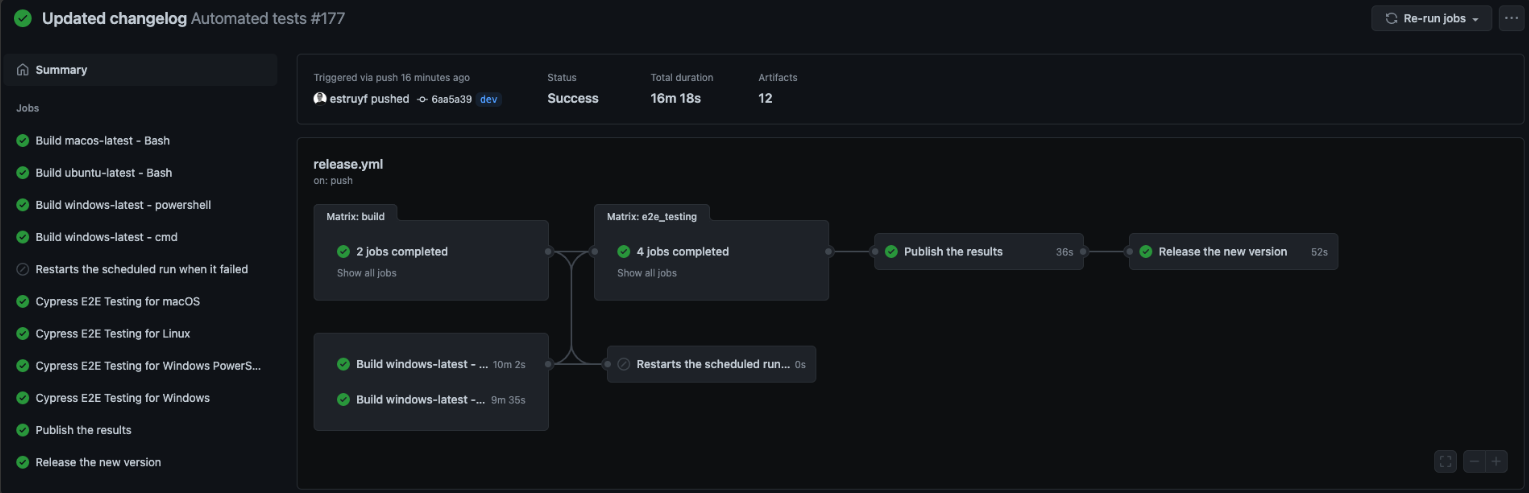
\includegraphics[height=0.2\textheight]{./part/Ejecucion/Seguimiento/PuestaAPunto/img/githubPipelines}
    \caption{Ejemplo de ejecución del Pipeline en Github para el despliegue del proyecto}\label{fig:githubActions}
\end{figure}

\subsubsection{Montaje del hardware}

Para probar el sistema dispone de un montaje Hardware, cuyo diagrama conceptual se puede ver en  figura~\cref{fig:despliegue de prueba}.
Cuyo aspecto real se puede ver en la~\cref{fig:montaje en protoboard}.
Muestra el montaje físico de conexión entre el el servidor cliente y el dispositivo controlado.
El servidor Raspberry se conecta mediante \textit{protoboard} realizando la conexión con el puente H y el motor de corriente continua.

\begin{figure}[H]
    \centering
    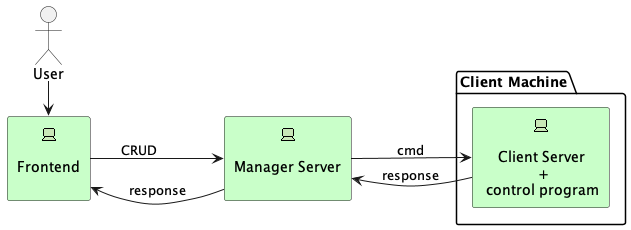
\includegraphics[height=0.2\textheight]{./part/Ejecucion/Seguimiento/PuestaAPunto/img/deploy}
    \caption{Diagrama de despliegue de prueba}\label{fig:despliegue de prueba}
\end{figure}

\begin{figure}[H]
    \centering
    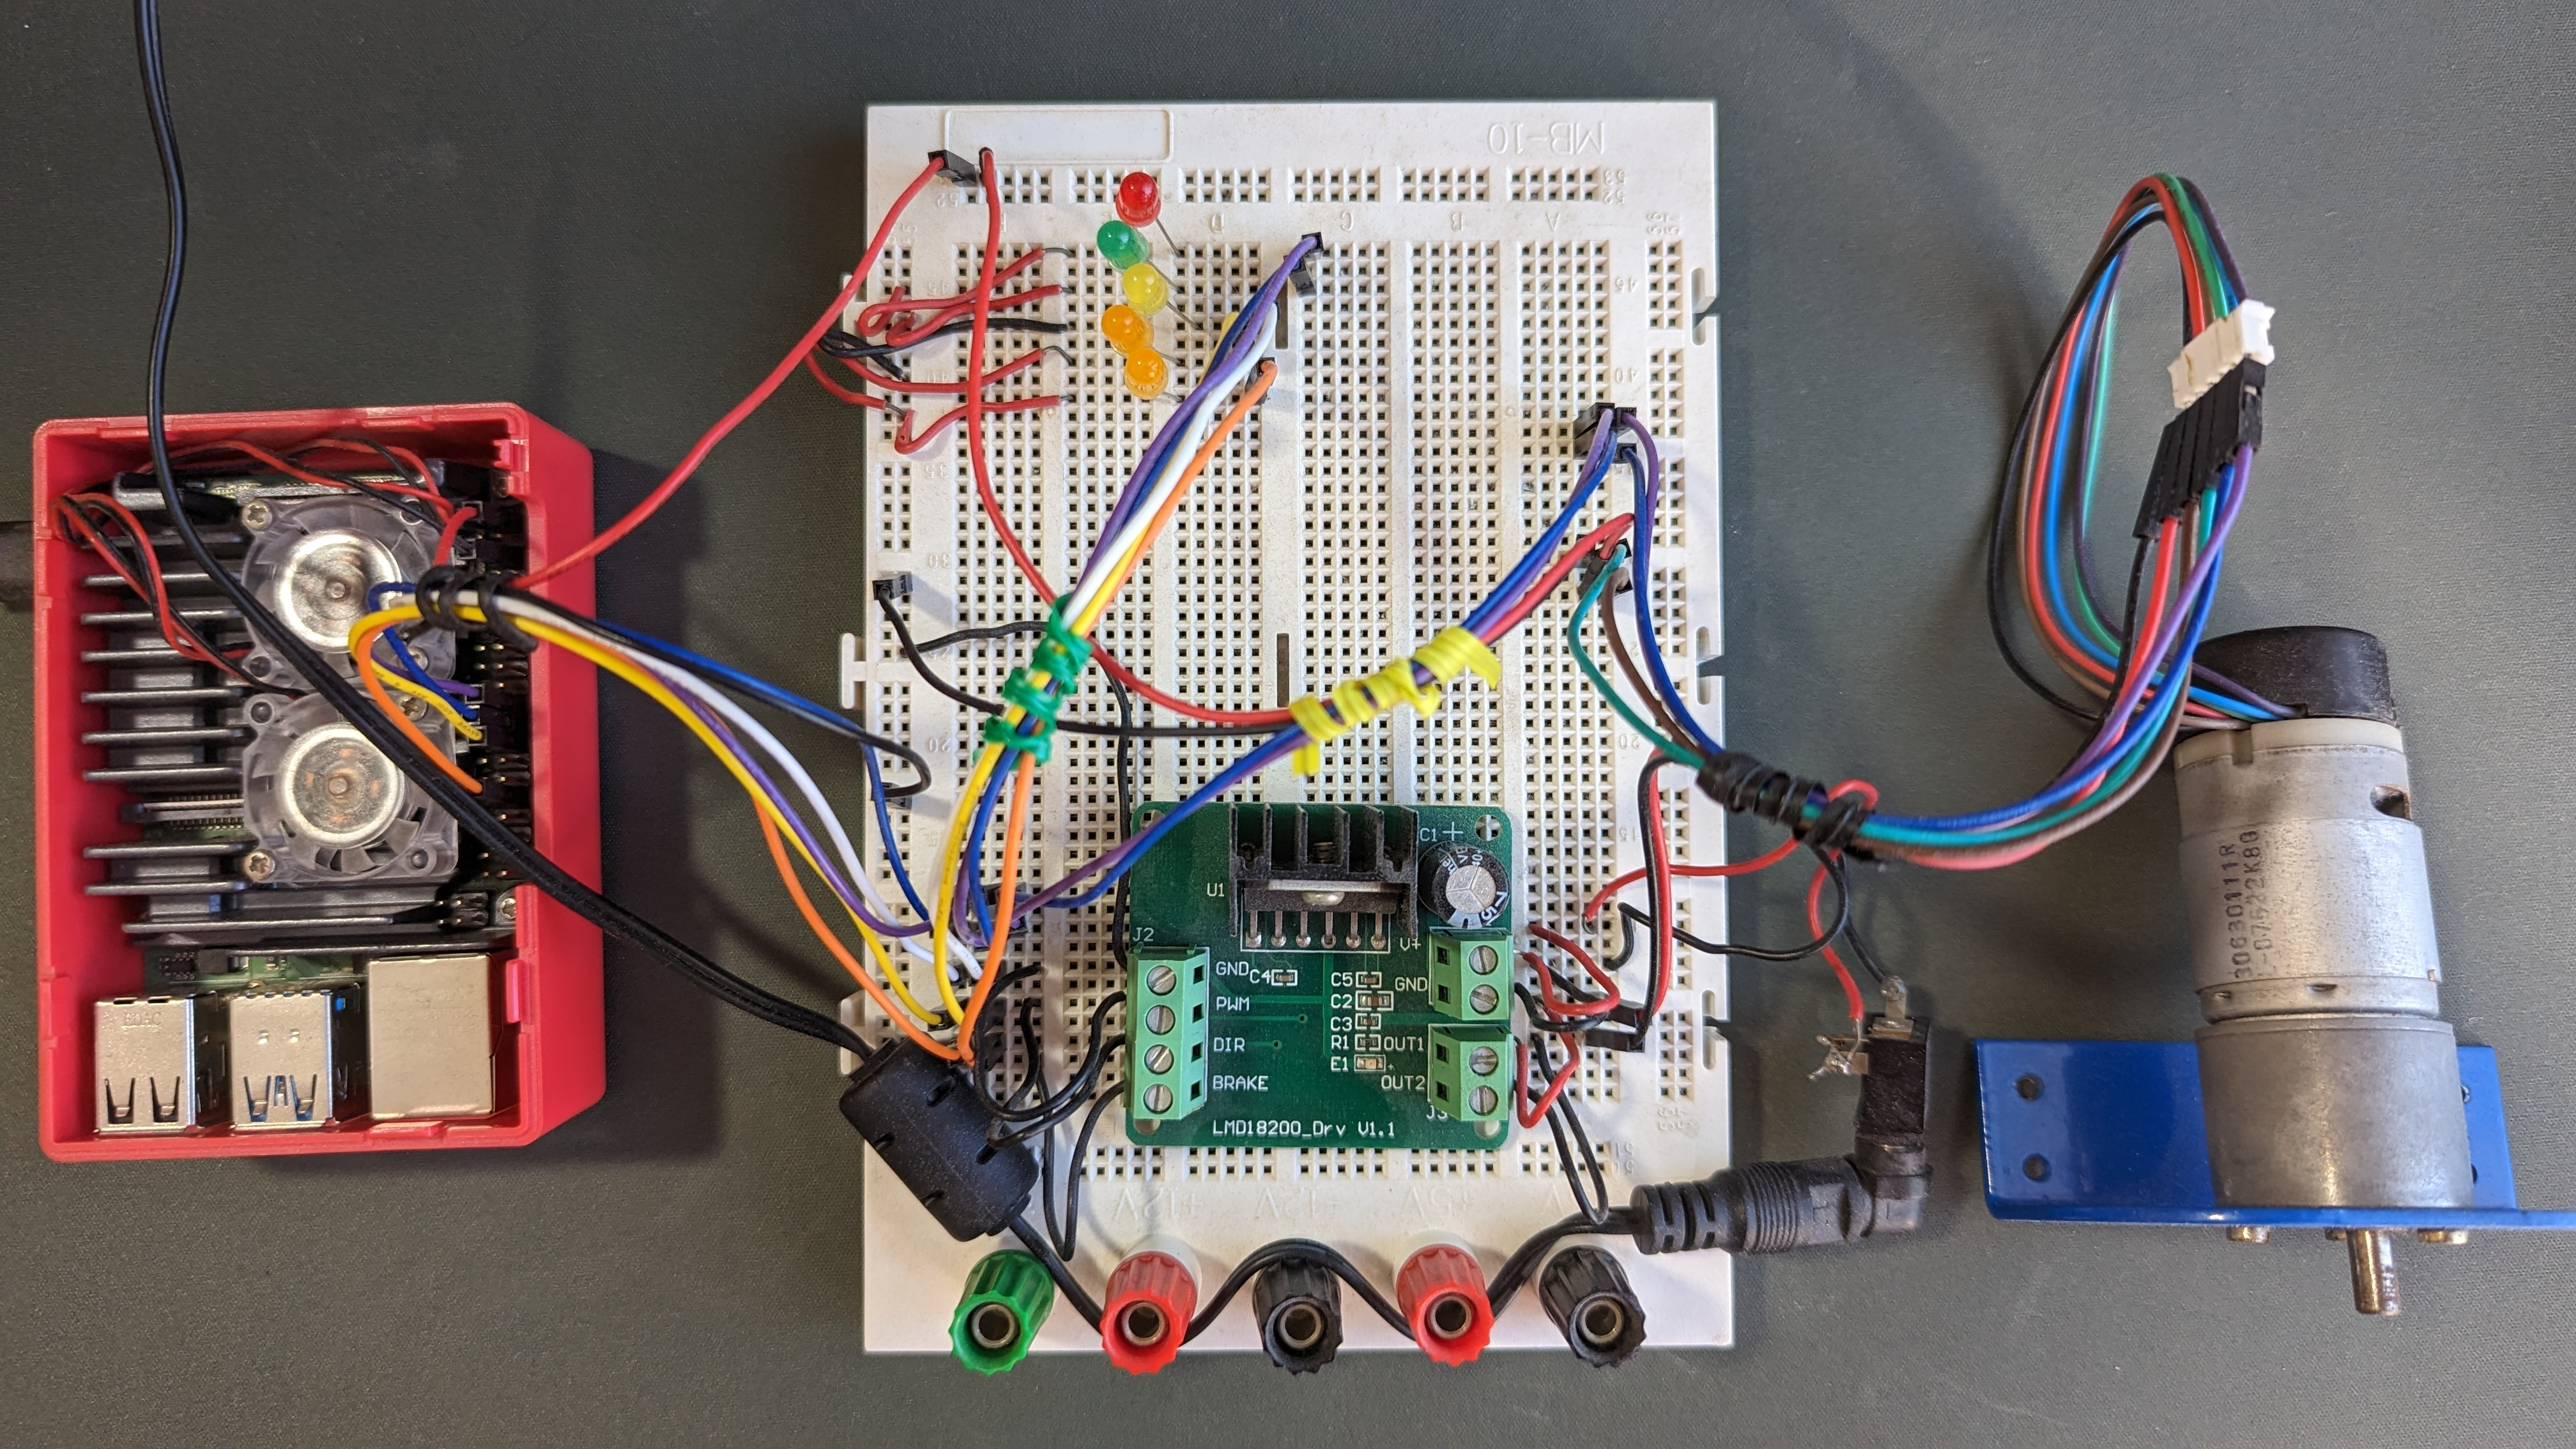
\includegraphics[height=0.2\textheight]{./part/Ejecucion/Seguimiento/PuestaAPunto/img/montajeProtoboard}
    \caption{Montaje en protoboard}\label{fig:montaje en protoboard}
\end{figure}

\subsubsection{Interfaz gráfica}

Para controlar el programa manager se ha desarrollado como añadido una interfaz gráfica.
No formaba parte de los objetivos del proyecto, pero se consideró que facilitaba el uso de la API disponible del programa Manager y la visualización de los resultados.
En la~\cref{fig:frontend} se muestra el aspecto del listado de las tareas creadas en el sistema.
Permite visualizar el estado en el que se encuentran y un botón para ejecutar manualmente las que disponen de dicha configuración.
Al ejecutar una tarea manual se dispone de una gráfica para ver en tiempo real la evolución de la variable controlada~\cref{fig:runner}.

\begin{figure}[H]
    \centering
    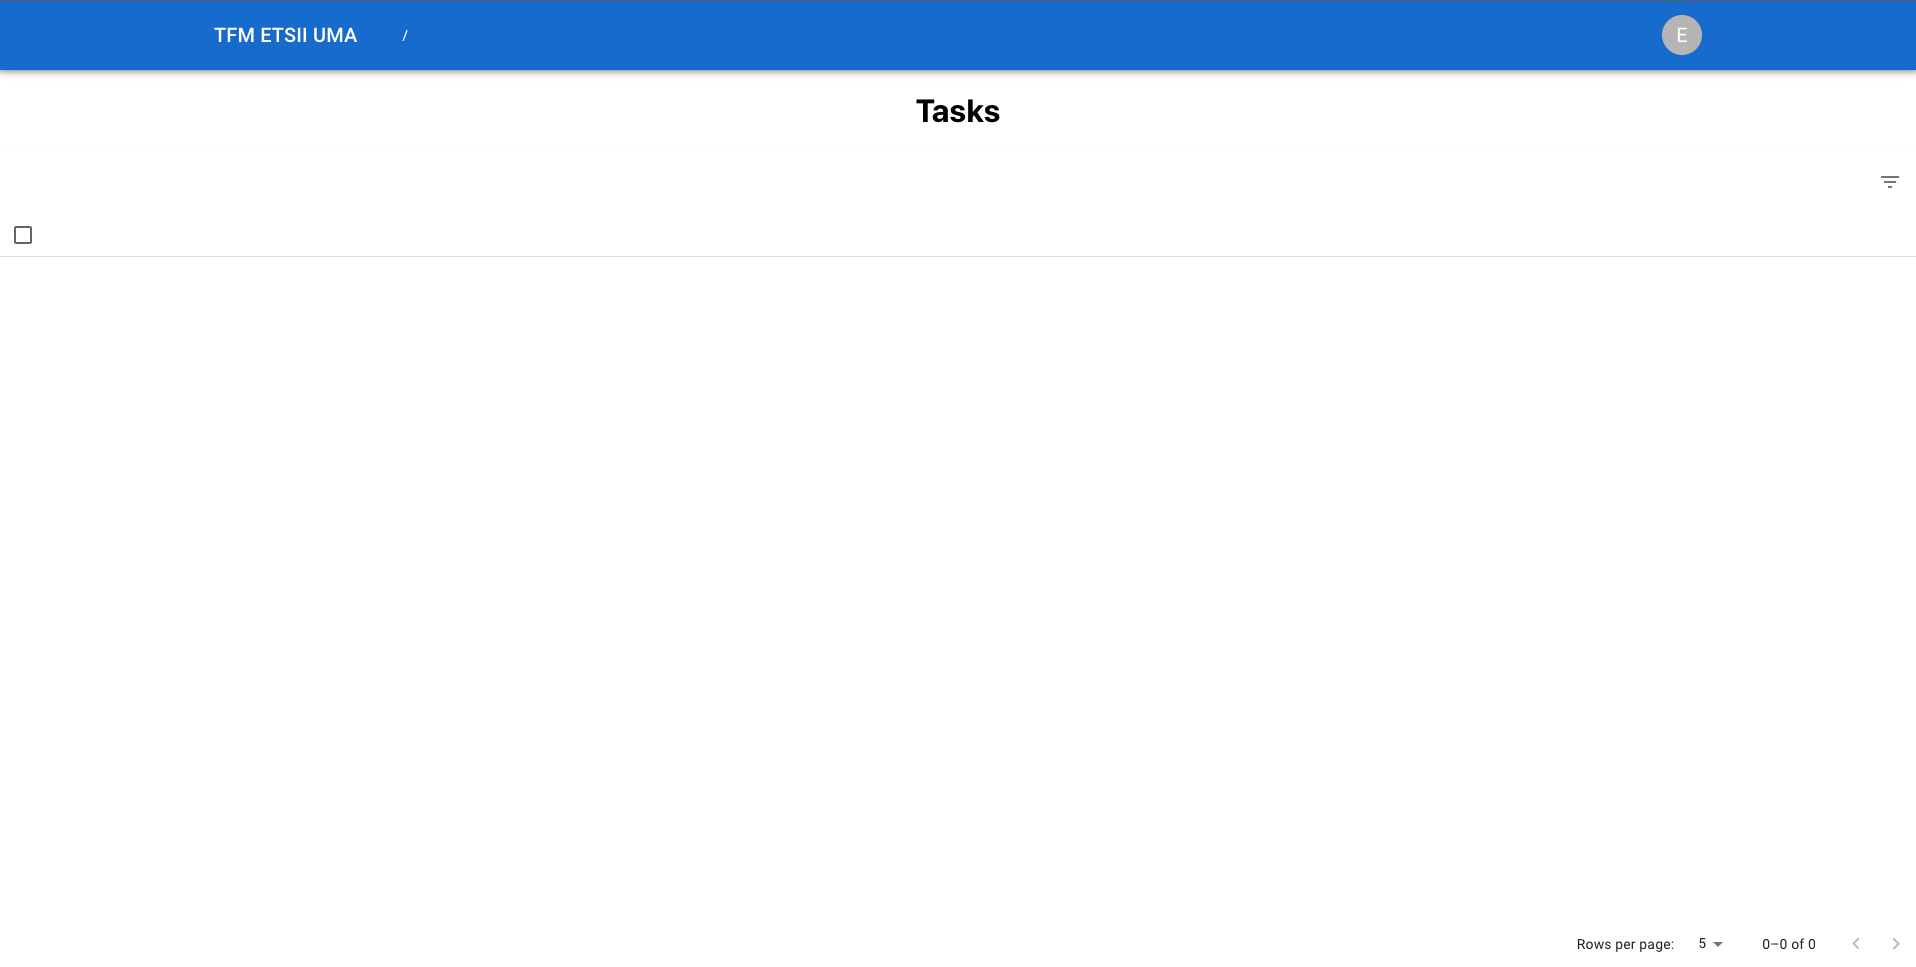
\includegraphics[height=0.2\textheight]{./part/Ejecucion/Seguimiento/PuestaAPunto/img/frontend}
    \caption{Frontend: task list}\label{fig:frontend}
\end{figure}

\begin{figure}[H]
    \centering
    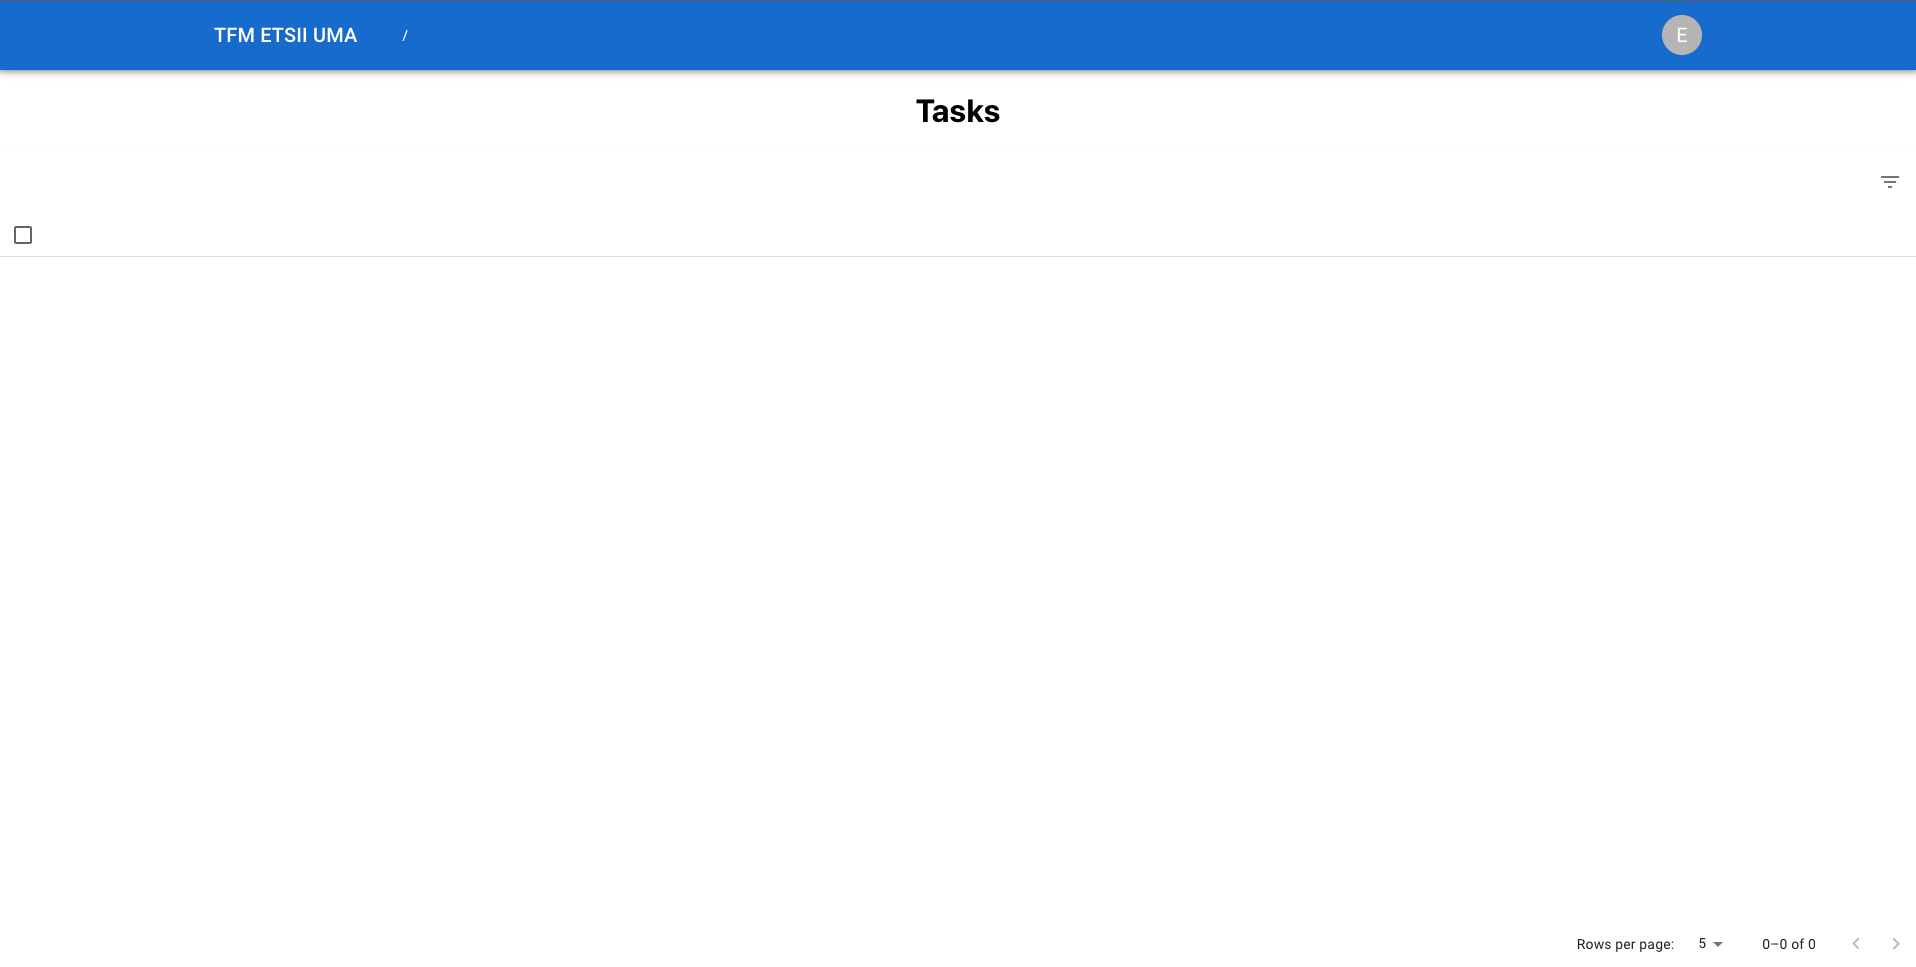
\includegraphics[height=0.2\textheight]{./part/Ejecucion/Seguimiento/PuestaAPunto/img/runner}
    \caption{Frontend: runner}\label{fig:runner}
\end{figure}

\subsubsection{Resultados}

Los resultados del control del Motor de corriente continua se muestran en la~\cref{fig:runner2}.
Se aprecia que para una consigna de 120 rpm, dos vueltas por segundo, el PID se estabiliza en torno al valor designado.

\begin{figure}[H]
    \centering
    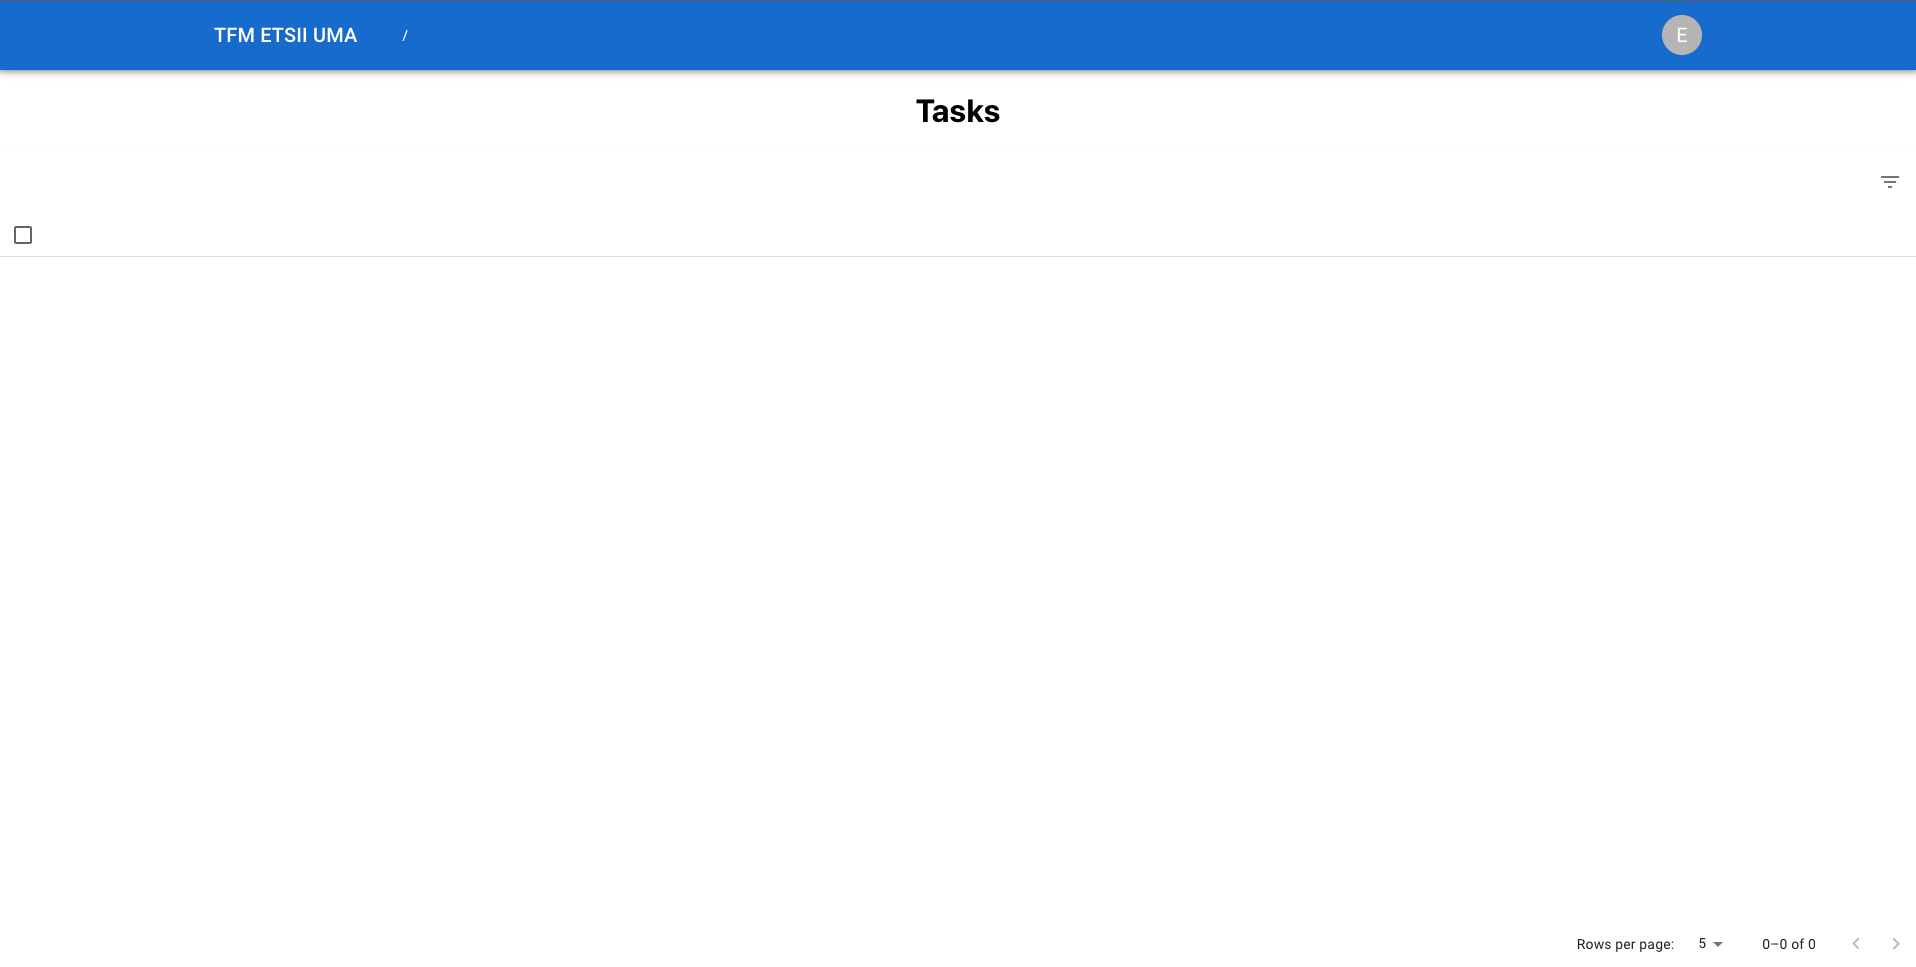
\includegraphics[height=0.2\textheight]{./part/Ejecucion/Seguimiento/PuestaAPunto/img/runner}
    \caption{Frontend: runner}\label{fig:runner2}
\end{figure}